When describing the Secure CC Protocol in Chapter \ref{cha:secure}, we referred to ``virtual credit cards''.
In this chapter, we describe them more formally.

\section{Virtual Credit Cards}

Many consumer smart phones today support the ability to communicate over the NFC channel.
Indeed, as described in Section \ref{sec:insecure-attacks}, this ability can be used by skimmers and relay attackers in order to perform fraudulent purchases.
Moreover, this ability can be used by an authorized party to perform non-fraudulent purchases.

A virtual credit card is an application on an NFC-capable smart phone, which emulates a credit card in a CC Protocol,
    by receiving Solicitation messages and responding with Card Information messages.
To emulate a physical credit card, the virtual credit card needs to have access to the following information:

\begin{itemize}
\item the credit card number
\item the expiration date
\item the next iCVV
\item the issuing bank name
\end{itemize}

Note that the credit card number, expiration date, and bank name can be input to the virtual credit card by the cardholder.
However, in order to be able to generate valid iCVVs, a virtual credit card must have access to the seed from which iCVVs are generated.
This value is not known to the cardholder, and as such, a virtual credit card cannot normally be created without the cooperation of the physical card's issuing bank.


\section{Electronic Wallets}
%There is no reason that a smart phone capable of NFC communication should be limited to supporting a single credit card.
A logical extension of the virtual credit card is the storage and management of multiple virtual cards in a single unit.
Applications such as Android Pay and Apple Wallet exemplify this idea,
    allowing a customer to use his smart phone to select the credit card with which to pay for a purchase,
    following which the phone emulates the selected credit card.
We refer to a collection of virtual credit cards and accompanying software
    (e.g. the interface for allowing the customer to select a card, password protection, etc.) as an ``Electronic Wallet''.
Figure \ref{fig:wallet} shows how an Electronic Wallet can be used in the CC protocols discussed so far
    (namely, the Insecure CC Protocol, the Externally Secure CC Protocol, and the Secure CC Protocol).
    enabling the customer to participate in the protocol as described in the Secure CC Protocol in Chapter \ref{cha:secure}.

\begin{figure}[h!]
  \caption{Use of an Electronic Wallet in the CC Protocols}
  \centering
    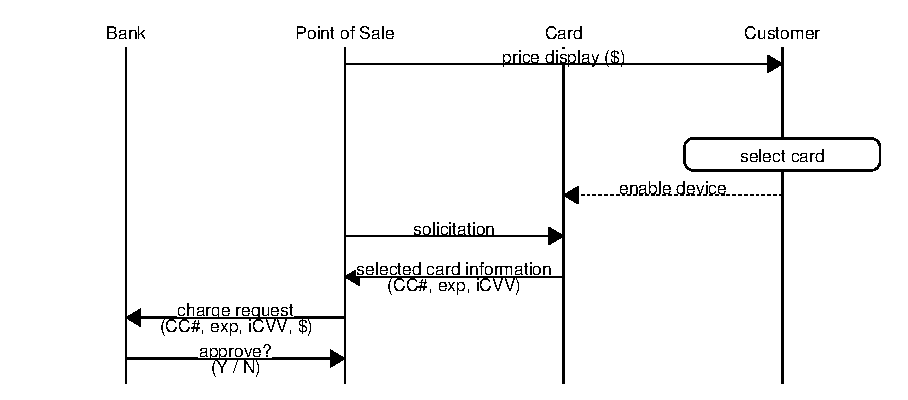
\includegraphics{img/wallet.eps}
  \label{fig:wallet}
\end{figure}

Electronic Wallets are advantageous for several reasons:
\begin{itemize}
\item Convenience: Electronic Wallets allow a customer to carry an essentially unlimited number of credit cards on their person without taking up extra space
\item Security: Electronic Wallets protect the customer from skimming and relay attacks,
    because Electronic Wallets are typically programmed not to respond to solicitations without customer consent.
    (Recall that physical credit cards will always respond to solicitation messages, regardless of the customer's intention.)
\item Interface: Electronic Wallets can provide a rich interface between the customer and the virtual credit card.
    This interface allows the customer to participate in the protocol.
\end{itemize}

Electronic Wallets will also be used in the Unlinkable CC Protocol, described in Chapter \ref{cha:unlinkable_design}.
